\chapter{Introduction}

The Jiangmen Underground Neutrino Observatory (JUNO), currently under construction in southern China, is a large liquid scintillator neutrino detector. It is designed to detect electron antineutrino interactions produced by nearby Nuclear Power Plants (NPP) through the inverse beta decay reaction. The primary objective of this experiment is to determine the neutrino mass hierarchy, thereby addressing the Neutrino Mass Ordering (NMO) problem.

The field of neutrino physics has entered a new era of precision following the measurement of the third lepton mixing angle, the so-called reactor angle $\theta_{13}$. This has had a significant impact on models of neutrino mass and mixing. The JUNO experiment, with its excellent energy resolution and large fiducial volume, is expected to make significant contributions to this field.

This leads us to the theory of neutrino oscillation, a quantum mechanical phenomenon whereby a neutrino created with a specific lepton flavor can later be measured to have a different flavor. The oscillation is quantified in terms of parameters that the JUNO experiment aims to measure with high precision.


\section{Neutrinos Oscillation}
The Standard Model of elementary particle interactions provides an accurate description of strong, weak, and electromagnetic interactions, but it treats these interactions as distinct and unrelated. Within this framework, neutrinos are assumed to be massless, but this assumption has been called into question by physicists. Neutrino oscillations, which occur when neutrinos change from one flavor to another, are a potential indication of neutrino mass.\\
The term "neutrino oscillations" refers to this phenomena and it involve the conversion of a neutrino of a particular flavor to another as it propagates through space.

Each known flavor eigenstate, $(\nu_e,\nu_{\mu},\nu_{\tau})$, linked to three respective charged leptons $(e,\mu,\tau)$  via the charged current interactions can be considered a complex combination of neutrino mass eigenstates as follow:

\begin{equation*}
	\left(\begin{array}{l}
		v_e \\
		v_\mu \\
		v_\tau
	\end{array}\right)=U_{\mathrm{PMNS}}\left(\begin{array}{l}
		v_1 \\
		v_2 \\
		v_3
	\end{array}\right)
\end{equation*}
in wich $\nu_i$ are the three mass eigensates, that have 3 masses  $m_i$  $(i = 1,2,3)$, which are non-degenerate, with $m_i \neq m_j$ for $i \neq j$.\\

The matrix $U_{\mathrm{PMNS}}$, called Pontecorvo-Maki-Nakagawa-Sakata (PMNS) matrix, is composed of three rotation matrices, $R_{23}$, $R_{13}$, and $R_{12}$, each corresponding to a different mixing angle, $\theta_{23}$, $\theta_{13}$, and $\theta_{12}$, respectively and a parameter $\delta_{CP}$ called the Dirac CP-violating phase. For this case, the Majorana $C P$ phases are $\eta_i(i=1,2)$, which are only physically possible if neutrinos are Majorana-type particles and do not participate in neutrino oscillations. Therefore, $U$ can be expressed as:

\begin{equation*} 
	\begin{split}
			U_{\text {PMNS }}&=\\
		=&\left(\begin{array}{ccc}
			1 & 0 & 0 \\
			0 & c_{23} & s_{23} \\
			0 & -s_{23} & c_{23}
		\end{array}\right) \left(\begin{array}{ccc}
			c_{13} & 0 & s_{13} \mathrm{e}^{-\mathrm{i} \delta_{C P}} \\
			0 & 1 & 0 \\
			-s_{13} \mathrm{e}^{\mathrm{i} \delta_{C P}} & 0 & c_{13}
		\end{array}\right) 
		\left(\begin{array}{ccc}
			c_{12} & s_{12} & 0 \\
			-s_{12} & c_{12} & 0 \\
			0 & 0 & 1
		\end{array}\right)\left(\begin{array}{ccc}
			\mathrm{e}^{\mathrm{i} \eta_1} & 0 & 0 \\
			0 & \mathrm{e}^{\mathrm{i} \eta_2} & 0 \\
			0 & 0 & 1
		\end{array}\right)
	\end{split}
\end{equation*}
where $s_{i j} \equiv \sin \theta_{i j}, c_{i j} \equiv \cos \theta_{i j}$.

The theoretical framework for neutrino oscillations involves the calculation of the oscillation probability as a function of the distance traveled by the neutrino, the neutrino mixing matrix, and the difference in squared masses between the three neutrino mass states, $\Delta m_{ij}^2 = m^2_i - m^2_j$ for $i,j = 1,2,3, i>j$ . Specifically, two nuclear power reactors 53 $\unit{\kilo\meter}$ away from the detector, which mostly produce anti-electron neutrinos $\bar{\nu}_e$ with energy below 10 MeV, are the principal sources of neutrinos for the JUNO experiment. So, it is necessary for the JUNO experiment to calculate the survival probability $P\left(\bar{\nu}_e \rightarrow \bar{\nu}_e\right)$ of electron antineutrinos.

\begin{equation*}
	P\left(\bar{\nu}_e \rightarrow \bar{\nu}_e\right)=1-\sin ^2 2 \theta_{12} c_{13}^4 \sin ^2\left(\frac{\Delta m_{21}^2 L}{4 \mathcal{E}}\right)-\sin ^2 2 \theta_{13}\left[c_{12}^2 \sin ^2\left(\frac{\Delta m_{31}^2 L}{4 \mathcal{E}}\right)+s_{12}^2 \sin ^2\left(\frac{\Delta m_{32}^2 L}{4 \mathcal{E}}\right)\right]
\end{equation*}

where $s_{i j} \equiv \sin \theta_{i j}, c_{i j} \equiv \cos \theta_{i j}, \mathcal{E}$ is the neutrino energy, $L$ the travelled distance and $\Delta m_{i j}^2 \equiv m_i^2-m_j^2$. \\
Past experiments have already given estimates for  $\Delta m_{21}^2,\left|\Delta m_{31}^2\right|$ and the  3 mixing angles.


\begin{figure}[h]
	\centering
	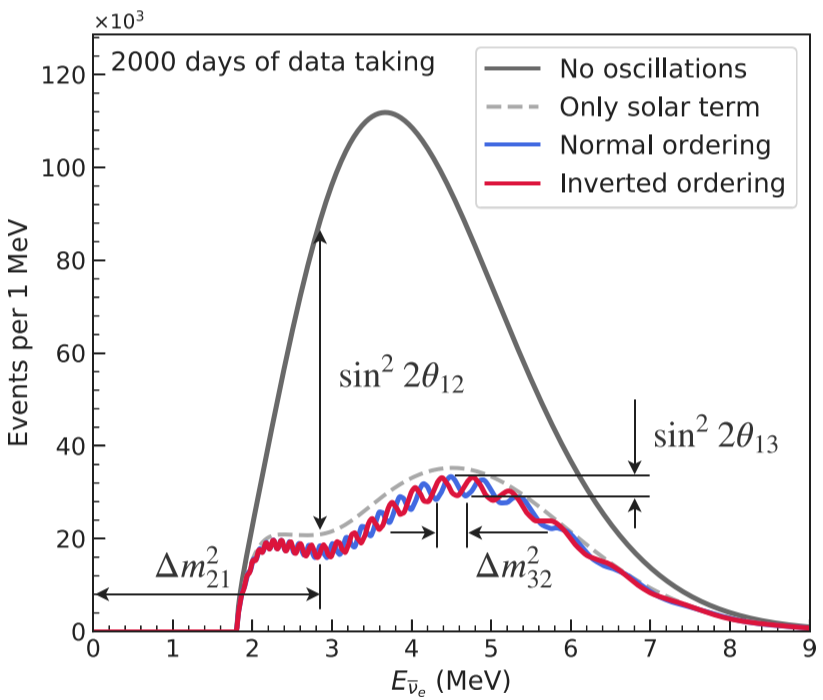
\includegraphics[width=0.3\linewidth]{Images/antineutino_to_antineutrino_probability_plot}
	\caption{JUNO's reactor antineutrino energy spectrum is shown with and without the effect of neutrino oscillation. The gray dashed curve includes only the term in the disappearance probability modulated by $sin^2(2\theta_{12})$, while the blue and red curves use the full oscillation probability for normal and inverted mass orderings. Spectral features driven by oscillation parameters are illustrated, highlighting the rich information available in JUNO's high-resolution measurement of the oscillated spectrum.}
	\label{fig:antineutinotoantineutrinoprobabilityplot}
\end{figure}


JUNO's primary objective is to refine these results, particularly to ascertain the sign of $\Delta m_{31}^2$, which will distinguish between two potential scenarios: Normal Ordering (NO), where $\left|\Delta m_{31}^2\right|=\left|\Delta m_{32}^2\right|+\left|\Delta m_{21}^2\right|$ and the mass hierarchy is $m_1<m_2<m_3$, and Inverted Ordering (IO), where $\left|\Delta m_{31}^2\right|=\left|\Delta m_{32}^2\right|-\left|\Delta m_{21}^2\right|$ and the mass hierarchy is $m_3<m_1<m_2$. The sign of $\Delta m_{31}^2$ subtly alters the plot of \ref{fig:antineutinotoantineutrinoprobabilityplot}. However, it remains uncertain whether the $\nu_3$ neutrino mass eigenstate is heavier or lighter than the $\nu_1$ and $\nu_2$ mass eigenstates.


\section{The JUNO detector}

Nestled beneath the Dashi hill in Jinji town, Southern China, the Jiangmen Underground Neutrino Observatory (JUNO) is an ongoing experiment. Its placement 43 km southwest of Kaiping city was strategically chosen to significantly reduce background noise from cosmic rays due to its underground location. JUNO is anticipated to detect a plethora of antineutrinos, predominantly originating from the Taishan and Yangjiang nuclear power plants (NPPs). These power plants are approximately 52.5 km away from the JUNO detector and together, they have a combined nominal thermal power of 26.6 $GW_{th}$. The detector's design has been meticulously optimized for the highest sensitivity to the ordering of neutrino masses.\\

Furthermore, the JUNO experiment deploys a specialized compact detector named TAO. Situated approximately 30 meters from one of the Taishan reactors, TAO serves to measure the unoscillated reactor antineutrino spectrum shape precisely. The data collected by TAO is intended to provide a crucial data-driven input to refine the spectra from the other reactor cores. The core of the JUNO detector, the \textbf{Central Detector (CD)}, is complemented by a water \textbf{Cherenkov detector} and a \textbf{Top Tracker (TT)}. Notably, the CD, designed as a compact, non-segmented detector, boasts an effective energy resolution of $\sigma_E/E =3\% / \sqrt{E (MeV)}$, a testament to the advantage of opting for a compact design over a segmented one.\\

The CD contains a 20 kton liquid scintillator (LS), safely housed within a spherical acrylic vessel and submerged in a water pool. The pool, with a diameter of 43.5 m and a height of 44 m, provides an adequate buffer to shield the LS from the radioactive influence of the surrounding rock.

The vessel is supported by a stainless steel (SS) structure through connecting bars. Additional CD PMTs are mounted on the inner surface of this structure, which also hosts compensation coils designed to mitigate the Earth's magnetic field and thereby minimize its impact on the photoelectron collection efficiency of the PMTs.

Above the water pool resides the Top Tracker, an assembly of a plastic scintillator array, meticulously arranged to measure muon tracks accurately. The CD is connected to the external environment through a chimney, which facilitates calibration operations. Located above this chimney is the Calibration House, equipped with special radioactivity shielding and a muon detector, playing a crucial role in the overall experimental setup.

A schematic illustration of both JUNO and TAO's location is presented in Fig. \ref{fig:junoschemeexperiment}.


\begin{figure}[h]
	\centering
	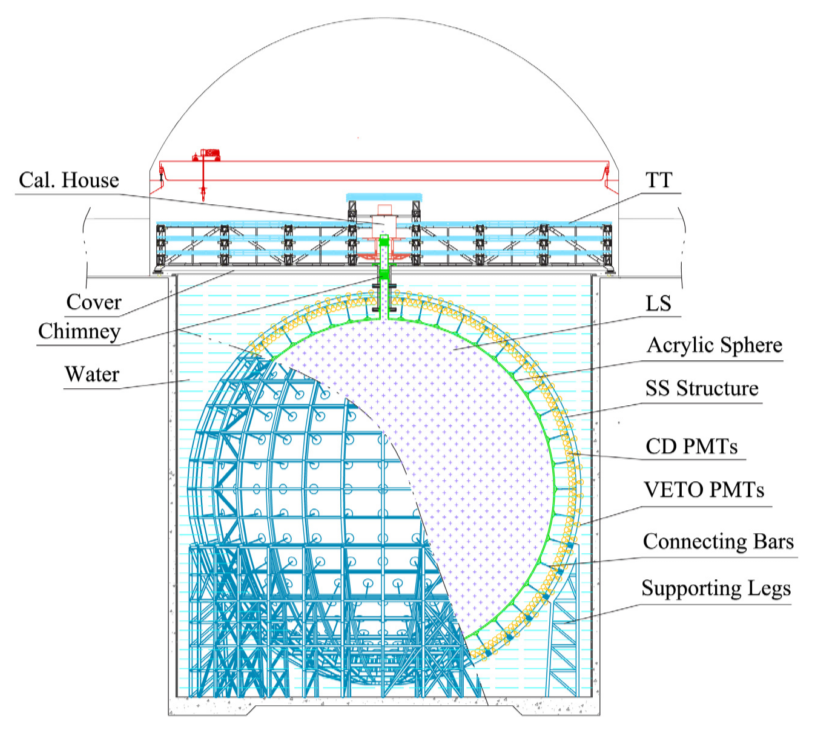
\includegraphics[width=0.7\linewidth]{Images/juno_scheme_experiment}
	\caption[JUNO scheme experiment]{Schematic view of the JUNO experiment}
	\label{fig:junoschemeexperiment}
\end{figure}


\section{JUNO signals and backgrounds}

\subsection{Signal}
%TODO: da qui in poi devi modificare
%LIQUID SCINTILLATOR

The primary ingredient of the LS is Linear Alkyl-Benzene (LAB) with a density of 0.859 $g/mL$. LAB is characterized by a straight alkyl chain of 10-13 carbons attached to a benzene ring, known for its remarkable transparency, high flash points, robust light yield, and low chemical reactivity, all critical factors in enhancing the detector's performance. The LS also contains 3 $g/L$ of 2,5-diphenyloxazole, serving as the fluor, and 15 $mg/L$ of p-bis-(o-methylstyryl)-benzene, which acts as the wavelength shifter. These ingredients, in collaboration with 17612 large 20-inch photomultiplier tubes (PMTs) and 25600 smaller 3-inch PMTs installed on a spherical structure with a 19.5 m radius, amplify the scintillation light signals, significantly contributing to the detection of neutrino events.

The scintillator is doped with a small amount of gadolinium to enhance its sensitivity to antineutrinos via the inverse beta decay (IBD) process. The liquid scintillator used in JUNO is a combination of LAB (linear alkyl benzene) and PPO (2,5-diphenyloxazole) doped with a small amount of bis-MSB (1,4-bis(2-methylstyryl) benzene). When a neutrino interacts with the scintillator, it can produce charged particles such as electrons, protons, and alpha particles that travel through the scintillator and excite the scintillation molecules. This excitation results in the emission of photons with a wavelength of around 430 nm. These photons are detected by 20,000 20-inch photomultiplier tubes (PMTs) distributed in a 3-dimensional arrangement inside the detector.\\




\begin{equation}
	\begin{aligned}
		\overline{\nu}e + p &\rightarrow e^+ + n \\
		n + ^A_ZX &\rightarrow ^{A}_{Z-1}X^* + \gamma \\
		e^+ + e^- &\rightarrow 2\gamma
	\end{aligned}
\end{equation} =

The PMTs detect the light and convert it into an electrical signal. The signals from all the PMTs are then combined to reconstruct the position and energy of the original neutrino interaction. This technique allows JUNO to measure the energy of the incoming neutrino to high precision, which is crucial for studying neutrino oscillation.

Moreover, the scintillator's composition and the detector's design are optimized to reduce background noise from other sources of radiation, such as cosmic rays and natural radioactivity. By carefully controlling these backgrounds, JUNO aims to achieve a signal-to-background ratio of better than 1:10,000, which is essential for observing the subtle effects of neutrino oscillation.

In JUNO's location, the energy spectrum will be distorted by two types of oscillations. The first is a slow (low frequency) oscillation driven by $\Delta m_{21}^2$ and modulated by $\sin ^2 \theta_{12}$, while the second is a fast (high frequency) oscillation driven by $\Delta m_{31}^2$ and modulated by $\sin ^2 \theta_{13}$. Fitting the data spectrum against the predicted spectrum distorted by standard neutrino oscillations enables measuring the oscillation parameters.\\
\subsection{Background}
Several different types of backgrounds signal are produced in the detector. For analysis we deeply analysed only the three most important contributes:


\paragraph{Radiogenic Backgrounds}

Radiogenic backgrounds arise from decays of radioactive isotopes in detector materials and surrounding rock. These decays can produce various forms of radiation, such as gamma rays and neutrons, which can interact with the detector and produce background events. Examples of radiogenic isotopes include $^{238}\mathrm{U}$, $^{232}\mathrm{Th}$, $^{40}\mathrm{K}$, and their daughter products. The main contributions to the radiogenic backgrounds come from the $^{238}\mathrm{U}$ and $^{232}\mathrm{Th}$ decay chains, with a smaller contribution from $^{40}\mathrm{K}$.

\paragraph{Cosmogenic Backgrounds}

Cosmogenic backgrounds arise from interactions of cosmic rays with materials surrounding the detector, such as the atmosphere and the Earth's crust. Muons produced in these interactions can penetrate the detector and produce background events. Specifically they interact with detector materials, producing isotopes such as $^{11}\mathrm{C}$, $^{9}\mathrm{Li}$, and $^{8}\mathrm{He}$, instable atoms which decay and produce additional background events.

\paragraph{Atmospheric Neutrino Backgrounds}

Atmospheric neutrino backgrounds arise from interactions of cosmic ray protons and nuclei with the Earth's atmosphere, which produce a flux of neutrinos that can interact with the detector. These interactions can produce both charged and neutral current events, which can mimic the signal from reactor neutrinos.

\paragraph{Reactor Antineutrino Backgrounds}

Reactor antineutrino backgrounds arise from the neutrinos produced in the nuclear reactors that power the JUNO experiment. These antineutrinos are the main signal for JUNO, but a small fraction of them can interact with the detector in ways that mimic background events. These interactions can produce both charged and neutral current events, which can be difficult to distinguish from the signal.


Here a viasualization sumary of all the bacgrounds contributions:

\begin{figure}[h]
	\centering
	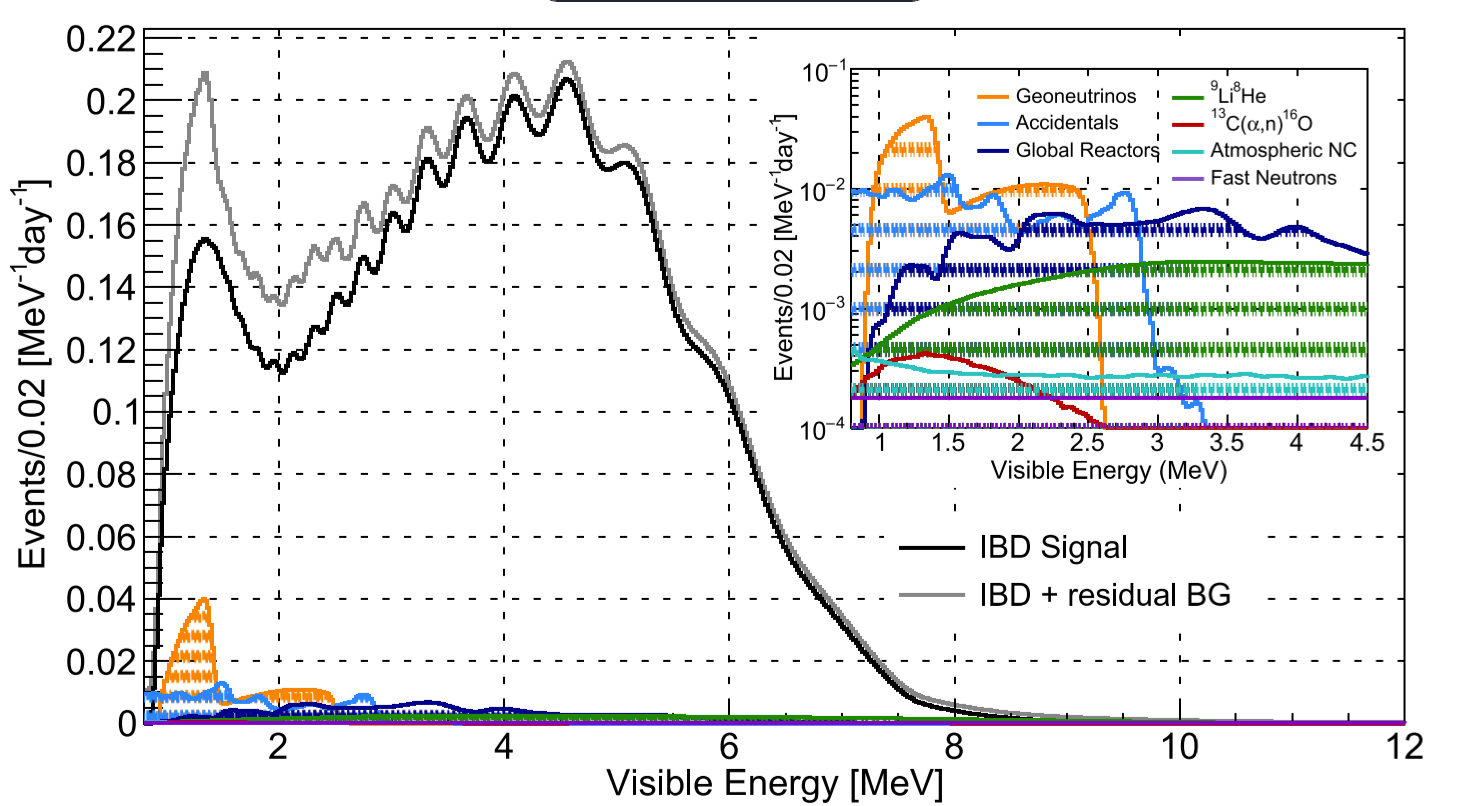
\includegraphics[width=0.7\linewidth]{Images/backgrounds_spectrum}
	\caption{Visible energy spectrum as measured by the LPMT system with (grey) and without (black) backgrounds is that which is anticipated for JUNO. The energy resolution is one of the assumptions listed in the text. The predicted backgrounds, which make up around 7$\%$ of the whole sample of IBD candidates and are primarily confined below, are shown in the inset as spectra. $\approx$ 3 MeV}
	\label{fig:backgroundsspectrum}
\end{figure}
